\section{Shared Process}\label{sec:crossTeam}

The definition of the development process of \gls{G19} resulted in a manual \cite{processManual} written by the \gls{ST}. The manual defines the practices and the work process to be followed by the \glspl{devTeam}.

The \gls{giraf} coordinator arranged a presentation by Anton Christensen, a student of \gls{G18}, where he described how his year had worked in teams which focused on one segment of the system. He raised concerns in working as they did in \gls{G18} as it made the developers very dependent on each other, which was shown to be troubling for the groups. \Gls{G19} decided to use another method, where the \glspl{devTeam} are \glspl{fullStack}, which means the \glspl{devTeam} work on the complete vertical slices rather than just on a single layer.

In order to achieve \glspl{fullStack} with the necessary information about the complete system, we introduced the idea of \glspl{skillGroup}, where we divide the system into three essential segments, namely frontend, backend, and server, which we can see in \autoref{fig:MetaGroupsFigure}. These groups make it possible for all \glspl{devTeam} to gain knowledge of all segments of the system. 

\begin{figure}[H]
        \begin{center}
            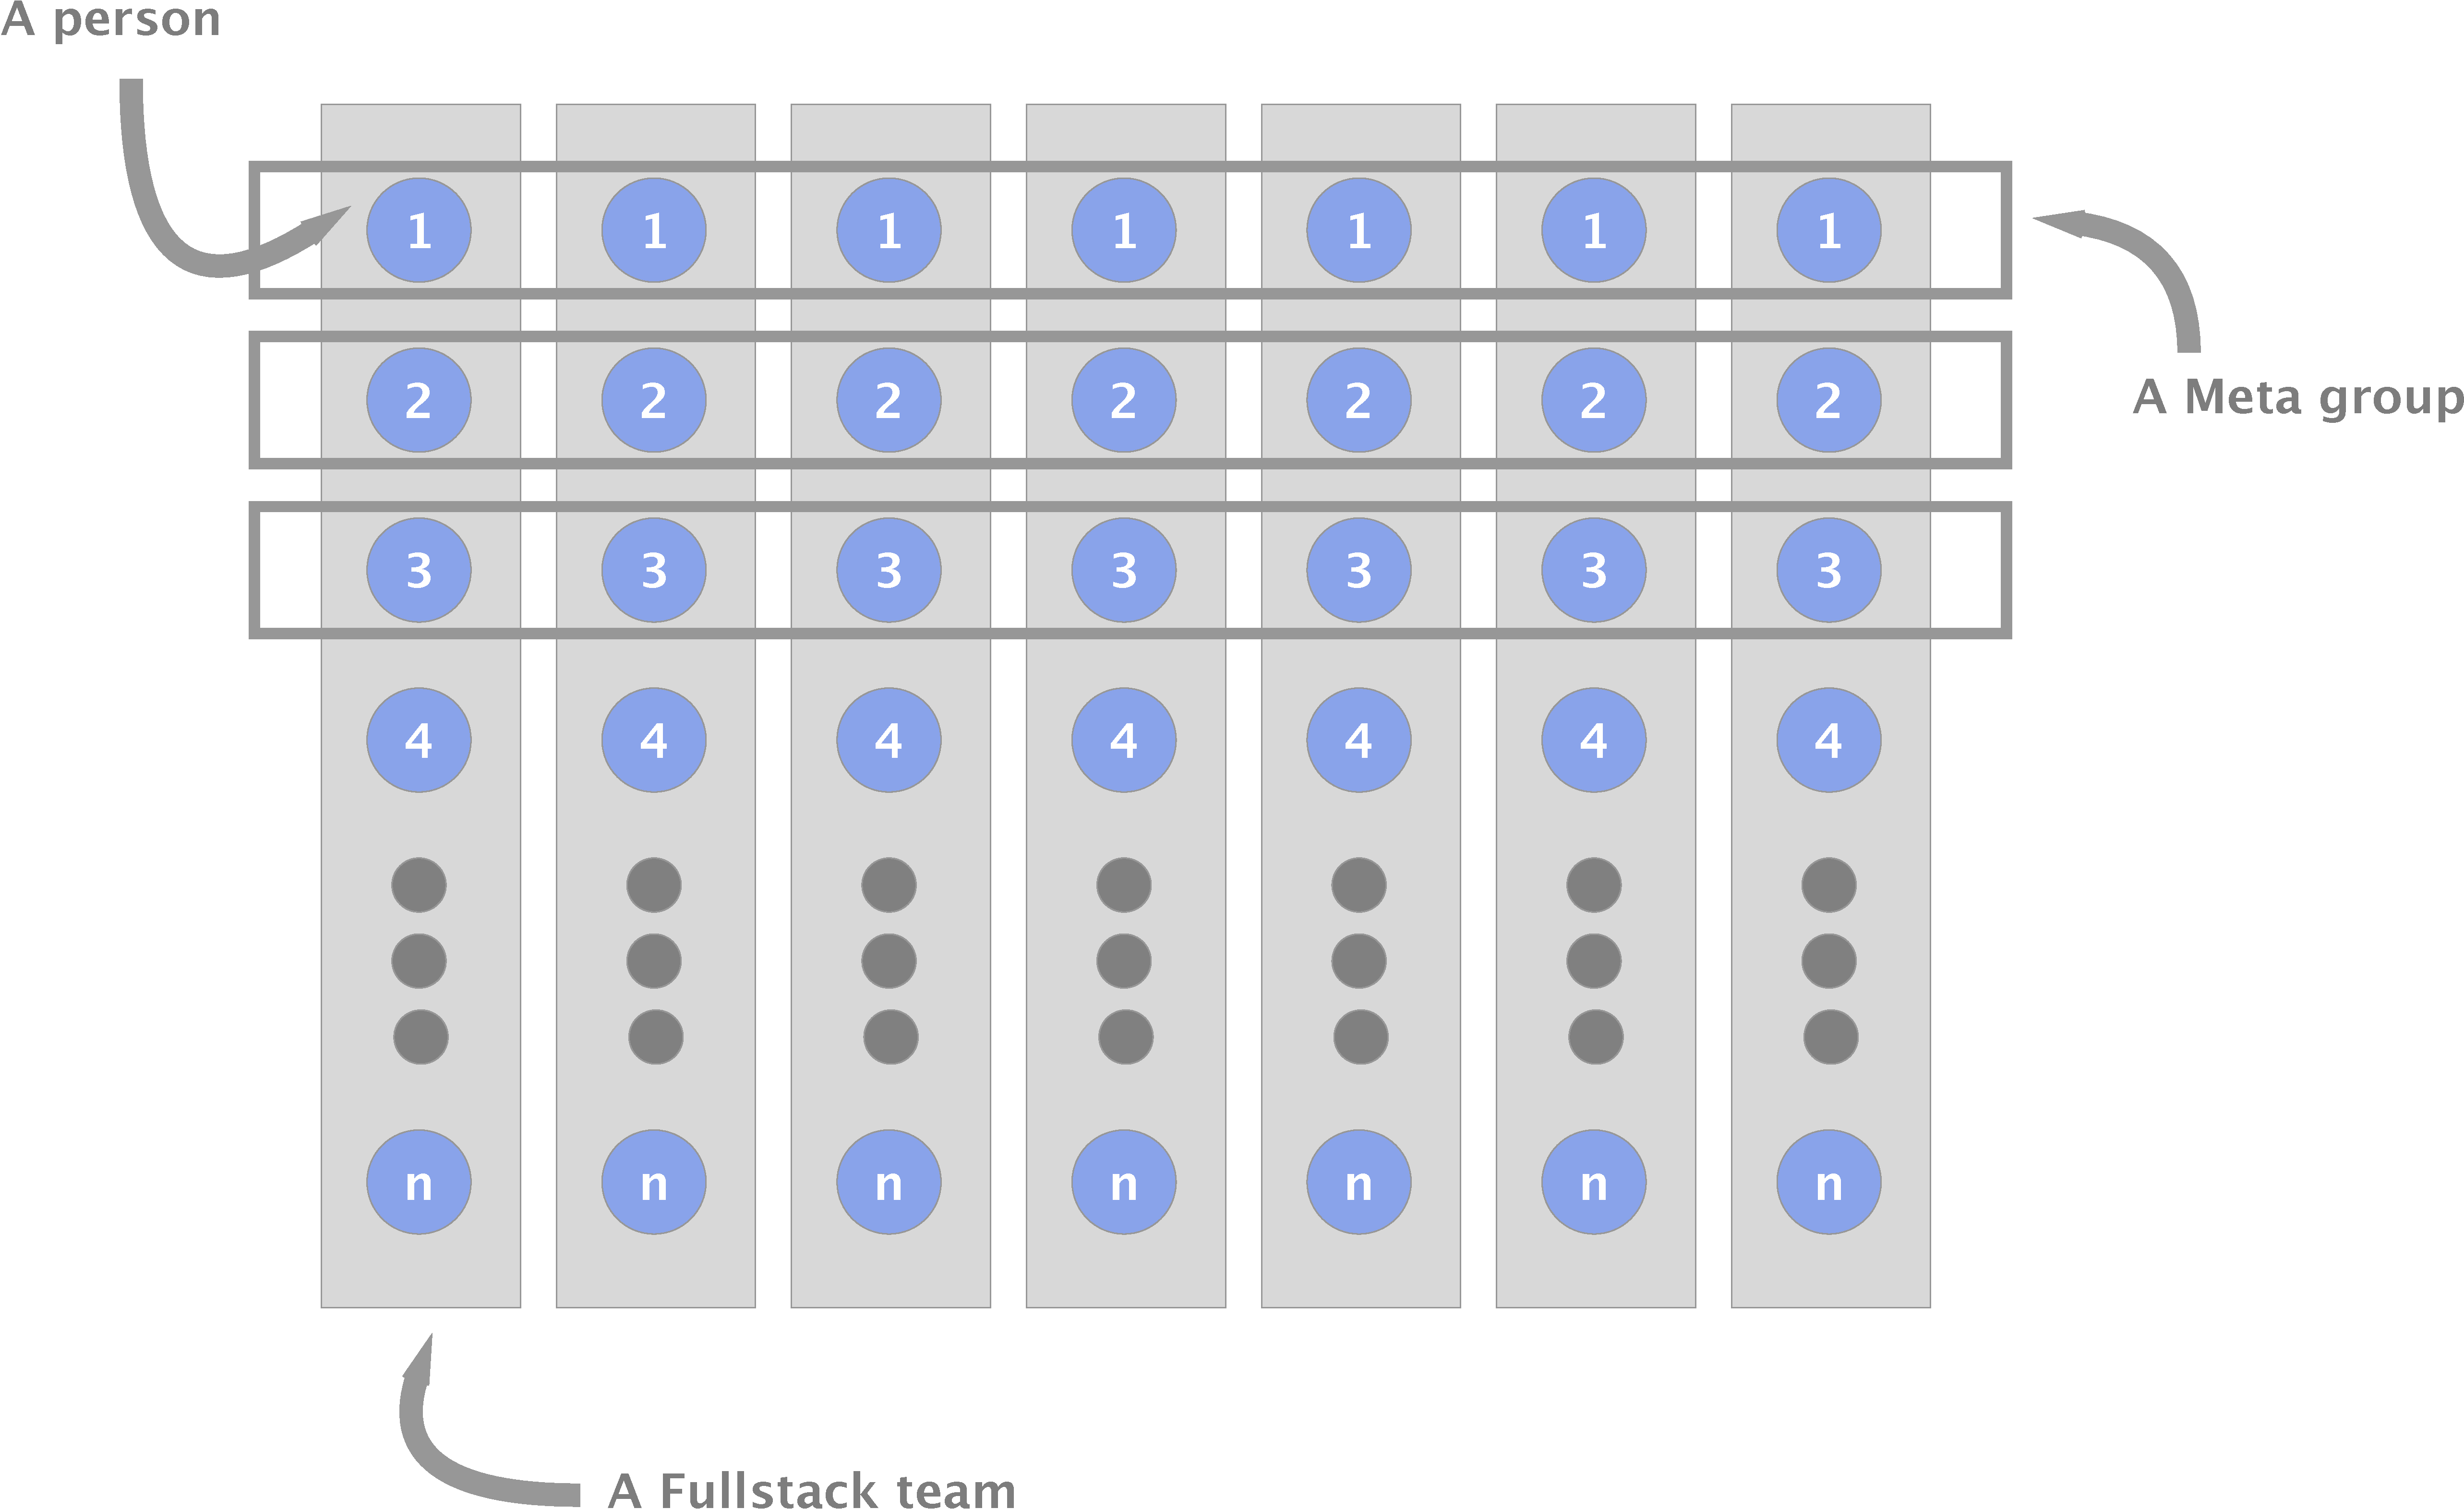
\includegraphics[width=0.95\textwidth]{figures/MetaGroupsFigure.pdf}
        \end{center}
        \caption{An illustration of how the \glspl{fullStack} and \glspl{skillGroup} are constructed}
        \label{fig:MetaGroupsFigure}
\end{figure}

\subsection{Process Activities}

The process selected for this semester was the \gls{SOS} process where the activities resemble the Scrum process where each group represents a team member.  Each \gls{devTeam} controls its internal work process. For an overview of the timeline of the activities within each sprint, see \autoref{fig:SprintTimeline}. This section describes the activities of the \gls{SOS} process, which are:

\begin{itemize}
    \item \Gls{SOSSprintPlanning}
    \item \Gls{SOSStandUp}
    \item \Gls{skillGroup} Meetings
    \item \Gls{ReleasePreparation}
    \item \Gls{SOSSprintRetrospective}
    \item \Gls{SOSSprintReview}
    \item Release Party
\end{itemize}

\begin{figure}[H]
        \begin{center}
            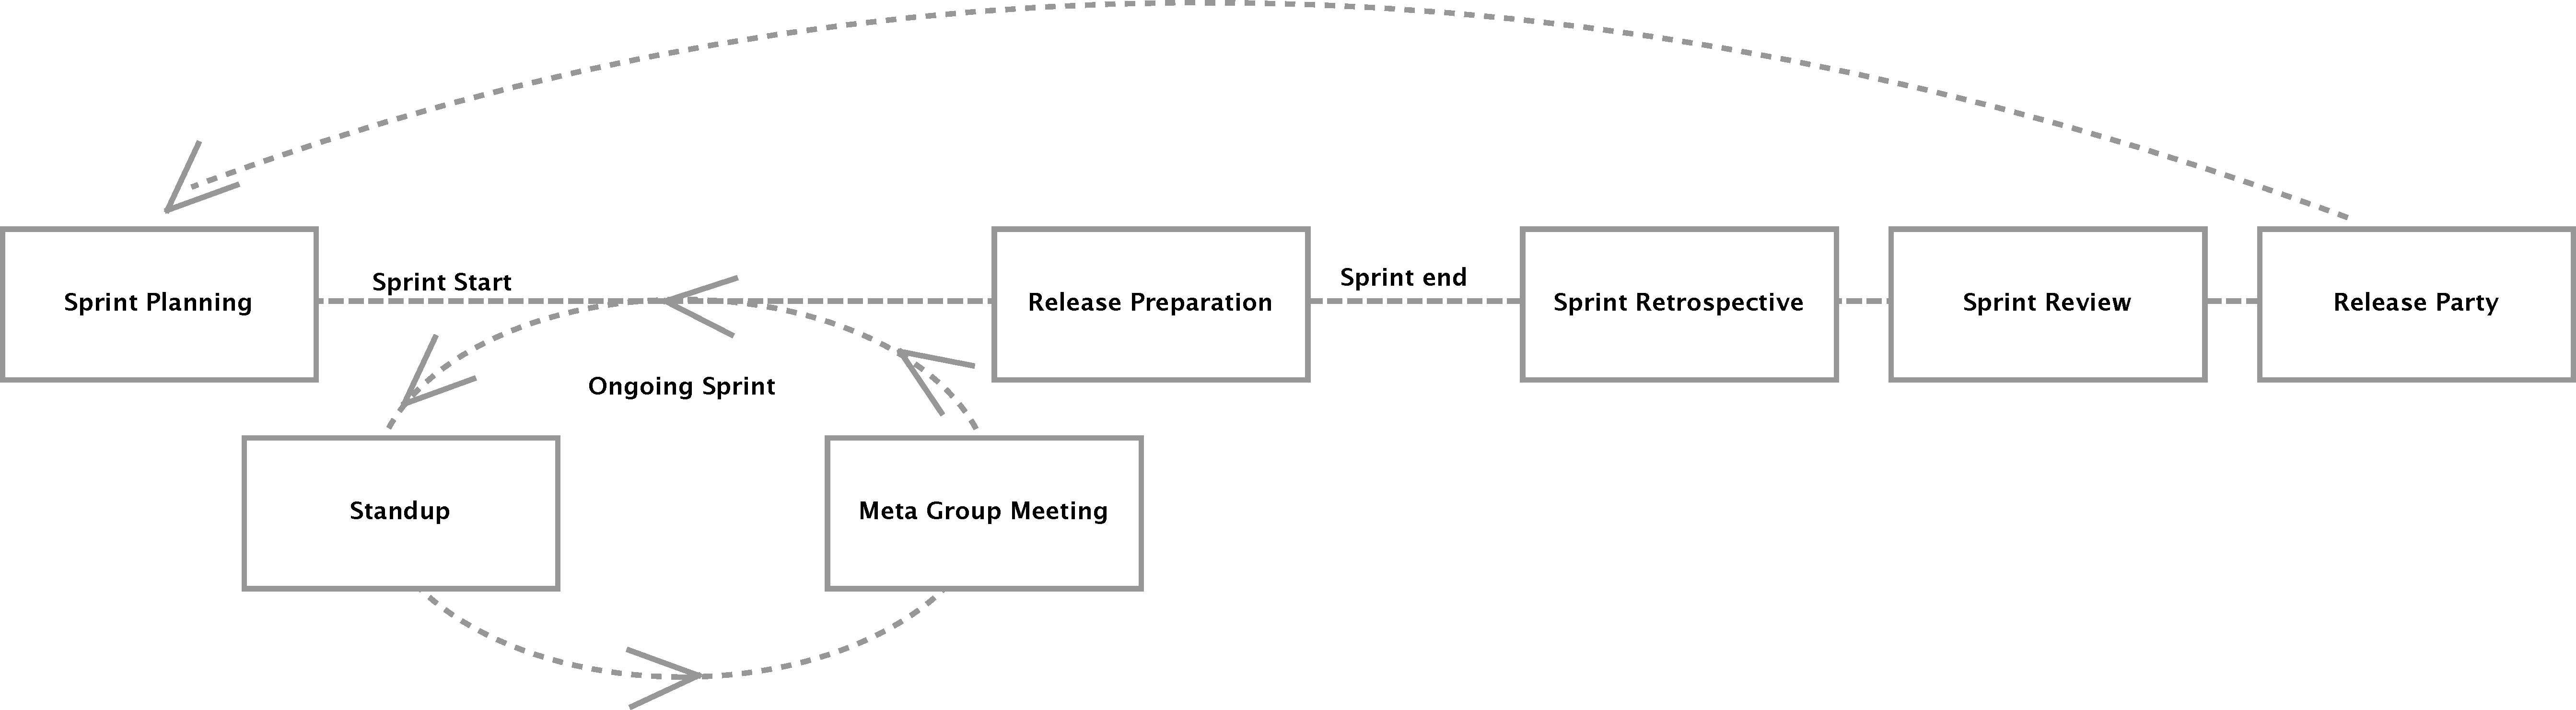
\includegraphics[width=1\textwidth]{figures/Process_overview.pdf}
        \end{center}
        \caption{The timeline of the activities in each of \gls{G19}'s sprints}
        \label{fig:SprintTimeline}
\end{figure}

\subsubsection{Sprint Planning}

Before a sprint ends, the \gls{POT} prepares the user stories for the next sprint, such that all members of \gls{G19} can plan the next sprint. The sprint planning begins with the \gls{POT} presenting the user stories to the \glspl{devTeam} along with the purpose of the sprint. The \glspl{devTeam} then choose the user stories which fit their team, consense the particular story with the \gls{PO}.

\subsubsection{Standup}

\Gls{SOSStandUp} is a status meeting, held one to three times a week, where one member from each \gls{devTeam} share their \gls{devTeam}'s progress and its challenges. The purpose of the meeting is to ascertain a shared state of the system and to help each other by raising concerns or answering questions. The meeting should not take more than 15 minutes.

\subsubsection{Meta Group Meetings}

There is a \gls{skillGroup} meeting for each segment of the system. The \gls{skillGroup} meetings are meant to make sure that every \gls{devTeam} is kept up to date with the progress of the different segments of the system as to aid their group members by answering any questions they might have. Every member of each \gls{skillGroup} go to their respective \gls{skillGroup} meeting, held at least once a week.

\subsubsection{Release Preparation}

\Gls{ReleasePreparation} covers four days before the end of each sprint. Here, the system is made ready for release, and the new features and changes are validated and verified.

\subsubsection{Review}

\Gls{SOSSprintReview} is held at the end of each sprint. Here, only one member from each group may attend. In this meeting, the \gls{PO} sums up the stories implemented throughout the sprint.

\subsubsection{Retrospective}

In the \gls{SOSSprintRetrospective} the development process is evaluated. Here, all members of \gls{G19} are to participate. Before the meeting, the \glspl{devTeam} should reflect on how they feel about the \gls{SOS} process. The members \gls{G19} divide themselves into reflection groups, containing approximately one member from each \gls{devTeam}. In these reflection groups, the participants discuss how they interpret their \gls{devTeam}'s experience with the current process. The \gls{ST} collects the feedback from each reflection group and tries to create a list of possible initiatives from the experiences. Afterward, we, \gls{G19} vote on the initiatives to emphasize the most important problems in the current process.

\subsubsection{Release Party}

The purpose of the Release Party is to improve the social bond between the \glspl{devTeam} and enhance the individual \gls{devTeam}'s involvement and ownership of the \gls{giraf} project. If a \gls{devTeam} wishes, they can present the user stories they have implemented.


